%Einleitung mit Motivation des Versuchs, Vergleich zu anderen hochauflösenden
%Mikroskopietechniken mit Literaturrecherche (ca. 1 Seite).
\subsection{Lichtmikroskopie}
STED-Mikroskopie ist eine Form der Lichtmikroskopie, die eine besonders gute Auflösung erreicht im Vergleich zu klassischen Mikroskopen.
Das klassische Lichtmikroskop basiert auf einem simplen Aufbau aus Linsen, wie er für einen einfachen Fall in Abb. \ref{fig:lightmic} zu sehen ist.
\begin{figure}
	\centering
	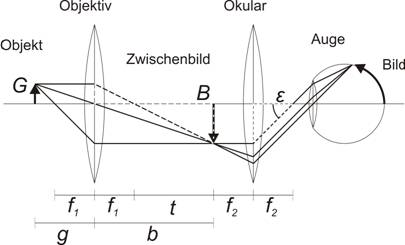
\includegraphics[width=0.6\textwidth]{plots/micro.jpg}\caption{Schematische Darstellung eines Zwei-Linsen Mikroskops aus. (Quelle: https://wiki.physik.fu-berlin.de)}\label{fig:lightmic}
\end{figure}
Im simpelsten Fall besteht wirft die erste Linse, das Objektiv, ein Bild in die Fokusebene der zweiten Linse, dem Okular \cite{Dem2}.
Der kleinst mögliche Abstand zweier Punkte unter dem noch zwei getrennte Punkte erkannt werden können ist die Auflösung des Mikroskops.
Sie ist bei der Lichtmikroskopie grundlegend durch Beugung beschränkt.
Beugung bewirkt, dass das Bild eines Punktes kein weiterer Punkt ist sondern eine mithilfe der Besselfunktion beschriebene Verteilung konzentrischer Ringe \cite{Born}, die sogenannte Punktspreizfunktion (PSF, \emph{point spread function}).
Insbesondere hat das Zentrum der Ringe, das erste Maximum, eine endliche Ausdehnung.
Dieses erste Maximum wird im Allgemeinen als Arrayscheibe bezeichnet.
\\
Das mit einem Mikroskop aufgenommene Bild einer Probe entspricht in seiner Form der Faltung der realen Form der Probe mit der PSF des Mikroskops.
Auf eine scharfe Kante wirkt diese Faltung als Glättung, sodass im Bild nur ein gradueller Übergang zu erkennen ist.
Die Wirkung der Faltung einer Kante mit einer Arrayscheibe ist in Abb. \ref{fig:convolution} schematisch dargestellt.\\
\begin{figure}
	\centering
	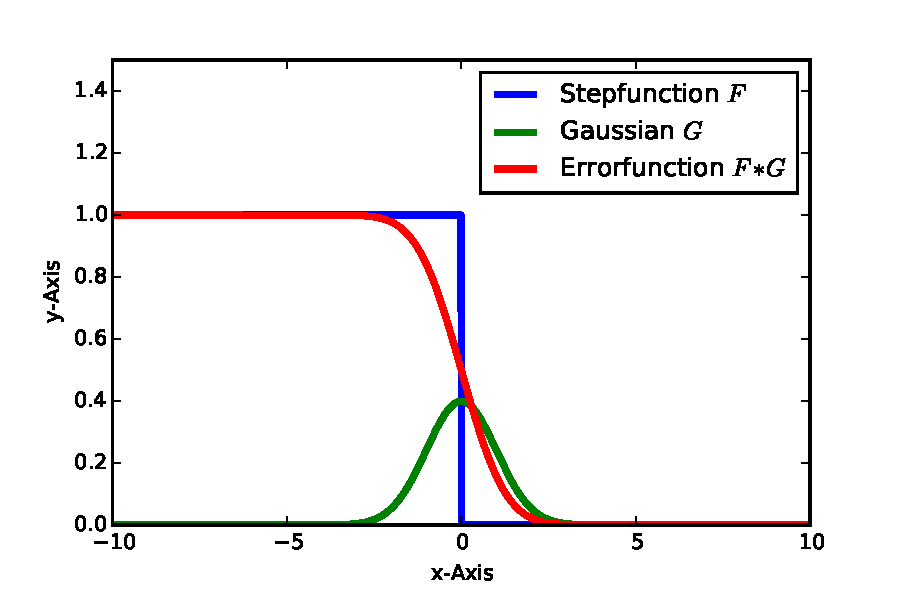
\includegraphics[width=0.75\textwidth]{plots/convolve.pdf}
	\caption{Faltung einer Kante (Stufenfunktion) mit einer Arrayscheibe (hier durch eine Gauß'sche Funktion genähert). Aus dem diskreten Sprung wird ein Gradient (in diesem Beispiel die Errorfunktion).}\label{fig:convolution}
\end{figure}
Liegen zwei Punkte zu dicht beieinander so überlappen sich ihre Arrayscheiben, und die Punkte können nicht mehr aufgelöst werden.\\
Die minimale Distanz, die zwei Punkte voneinander haben müssen, um als zwei Punkte erkannt zu werden, wird durch Auflösungskriterien bestimmt.
Das Sparrow'sche Auflösungskriterium \cite{sparrow} besagt, dass zwei Punkte (im Original Sterne) dann noch aufgelöst werden können, wenn die Intensitätsverteilung zwischen zwei Maxima gerade noch ein Minimum aufweist.
Eine konservativere Definition eines Auflösungskriteriums ist hingegen das Rayleighkriterium, welches in diesem Versuch hauptsächlich benutzt wird.
Nach Rayleigh werden zwei Punkte genau dann noch aufgelöst, wenn das Maximum eines Punktes in das Minimum des anderen fällt \cite{Dem2}.
Dies entspricht dem Abstand des ersten Minimums der PSF vom ersten Maximum und ist gegeben durch die Formel \ref{eq:rayleigh}
\begin{align}
	d_{min} = 1.22\cdot \frac{\lambda}{2n\sin \alpha}. \label{eq:rayleigh}
\end{align}
Hierbei beschreibt $\lambda$ die Wellenlänge des zu Mikroskopieren verwendeten Lichts, $n$ den Brechungsindex des Mediums und $\alpha$ den maximalen Öffnungswinkel der Obejktivlinse.
Der Term $n\sin\alpha$ wird als die numerische Apertur eines Objektivs $NA$ bezeichnet \cite{Born}.
\\
Experimentell ist die Auflösung nach Rayleigh oder Sparrow nur schwer zu messen. 
Als Maß für die Auflösung kann jedoch die Halbwertsbreite der PSF (FWHM, \emph{full width at half maximum}) benutzt werden. 
%• Erklärung Fluoreszenz und Fluoreszenzmikroskopie mit Jablonski-Diagramm.
\subsection{Fluoreszenzmikroskopie}
\begin{figure}
	\centering
	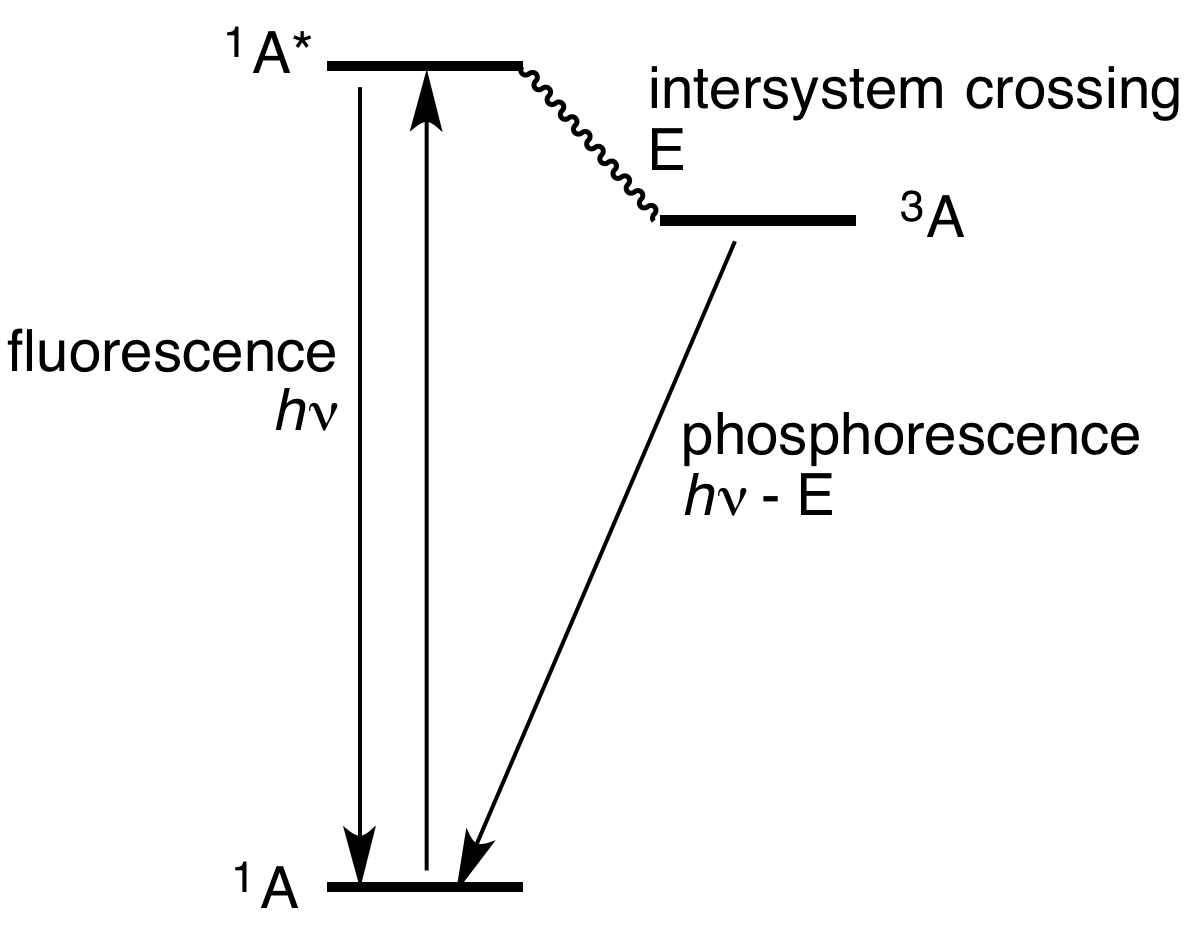
\includegraphics[width=0.6\textwidth]{plots/jablonski.png}
	\caption{Jablonski-Diagramm. (Quelle: en.wikipedia.org)}\label{fig:jablonski}
\end{figure}
Eine besondere Art von Lichtmikroskopie ist die Fluoreszenzmikroskopie.
Im Gegensatz zur klassischen Mikroskopie wird nicht, das von der Probe reflektierte oder an der Probe gebrochene Licht im Okular detektiert, vielmehr wird die Probe selbst zum Leuchten angeregt.
Das Prinzip der Fluoreszenz besteht darin Moleküle mithilfe von Licht einer spezifischen Wellenlänge in einen energetisch höheren Zustand zu versetzen. 
Bei der Rückkehr der Moleküle in ihren Grundzustand senden diese Photonen aus. 
Die Wellenlänge der absorbierten und emittierten Photonen hängt von der Verteilung der Energieniveaus des Moleküls ab. Sie ist in sogenannten Jablonski-Diagrammen schematisch dargestellt (siehe Abb. \ref{fig:jablonski}).
In der Regel befindet sich ein angeregtes Molekül nicht nur in einem elektronisch angeregten Zustand sondern auch in einem angeregten Schwingungszustand.
Durch die Relaxation aus dem Schwingungszustand besitzt das Molekül eine geringere Energie vor der Emission eines Photons als unmittelbar nach der Anregung.
Dies führt dazu, dass emittiertes Licht eine größere Wellenlänge hat als absorbiertes Licht. Dieses Phanomen trägt den Namen Stokes-Shift \cite{haken}.
\\
Der Vorteil der Fluoreszenzmikroskopie gegenüber der herkömmlichen Lichtmikroskopie ist, dass gezielt Strukturen mit Fluoreszenzfarbstoff präpariert werden können (über Proteine u.ä.) und ungewollte Brechungszentren ausgeblendet werden können.
Durch im Strahlengang eingesetzte Farbfilter wird gewährleistet, dass lediglich die emittierte Wellenlänge in das Objektiv gelangt und reflektiertes Licht abgeschrimt wird.
%• Konfokal-Mikroskopie: gehen Sie hier bitte kurz auf die Rolle der Lochblende ein
\subsection{Konfokalmikroskopie}
Eine Form der Fluoreszenzmikroskopie ist die Konfokalmikroskopie. 
Konfokalmikroskopie beleuchtet meist mit einem fokusierten Laser nur einen kleinen Ausschnitt der Probe. Allerdings wird die gesamte Probe abgerastert, sodass erst nach dem Zusammenfügen der einzelnen Flecken ein vollständiges Bild entsteht.
\\
Das Besondere an der Konfokalmikroskopie ist eine im Detektionsstrahlengang eingebrachte Lochblende. Ihre Funktion ist die Abschirmung von Licht, welches nicht von der Fokusebene stammt. Dadurch ist es möglich einen hohen Kontrast zu erzielen und nur einen scharfen Ausschnitt einer Ebene der Probe aufzunehmen.
\\
Die axiale Auflösung eines Konfokalmikroskops ist durch Gleichung (\ref{eq:axial}) bestimmt \cite{beyer}.
\begin{align}
	d_{axial} = \frac{0.88\cdot \lambda_{ex}}{n-\sqrt{n^2-NA^2}}. \label{eq:axial}
\end{align}
Hier bezeichnet $\lambda_{ex}$ die Wellenlänge der Fluoreszenzanregung. 
Die Dicke der beleuchteten Schicht lässt sich nach Gleichung (\ref{eq:slice}) bestimmen \cite{beyer}.
\begin{align}
	d_{schicht} = \sqrt{\left( \frac{0.88\lambda_{ex}}{n-\sqrt{n^2-NA^2}}\right)^2 + \left( \frac{\sqrt{2}\cdot n \cdot PH}{NA}\right)^2}. \label{eq:slice}
\end{align}
$PH$ bezeichnet den Durchmeser der konfokalen Lochblende.
%und nennen die zu erwartende Tiefendiskriminierung.
%• Beugungsgrenze in der Mikroskopie, Airy-Scheibe, beugungsbegrenzte PSF (rigo-
%rose Herleitung nicht nötig!), die Sie später für die Auswertung benötigen, Auflö-
%sungskriterien Rayleigh, Sparrow und axiale Auflösung.
%• STED-Mikroskopie: Erklärung des zugrundeliegenden Prinzips zur Auflösungs-
%erhöhung mit eigenen Worten (wichtig!).
\subsection{STED-Mikroskopie}
Die STED-Mikroskopie bietet eine Möglichkeit, die ansonsten in der Lichtmikroskopie auftretende Begrenzung der Auflösung durch Beugung zu umgehen.
Sie basiert auf der Fluoreszenzmikroskopie, und wird häufig mit einem konfokalen Aufbau realisiert.
\\
STED steht für \emph{stimulated emission depletion}, und bezieht sich auf die Abregung von Fluoreszenzmolekülen durch das Prinzip der stimulierten Emission. 
Im Gegensatz zur konventionellen Fluoreszenzmikroskopie, kommen zwei Laser unterschiedlicher Wellenlängen zum Einsatz \cite{hell}. 
Der Anregungslaser verfügt über eine PSF wie sie auch in der herkömmlichen Konfokalmikroskopie angewendet wird, i.e. eine gewöhnliche Airyscheibe.
Hinzu kommt nun ein Abregungslaser oder STED-Laser, dessen PSF die Form eines Ringes hat. Die Wellenlänge des STED-Lasers ist dabei größer als die des Anregungslasers.
Die PSFs beider Laser sind so überlagert, dass das Maximum der Anregung im Mittelpunkt des Ringes liegt.
\\
Der Anregungslaser regt Moleküle auf ein höheres Energieniveau an, die daraufhin unter Aussendung von Photonen wieder in ihren Grundzustand zurückkehren.
\\
Durch stimulierte Emission, lässt sich die Photonemission einer spezifischen Wellenlänge kontrolliert herbeiführen.
Interagiert ein angeregtes Elektron des Moleküls mit einem Photon dessen Wellenlänge dem Übergang zu einem niedrigeren Energieniveau entspricht, so fällt das Elektron in diesen Zustand unter Aussendung eines weiteren Photons dieser Wellenlänge.
\\
Dieses Prinzip wird durch den STED-Laser angewendet. Dadurch werden Moleküle aus dem Ring wieder abgeregt.
Da die Moleküle jedoch in der Regel in einen vibronischen Zustand fallen, können diese nicht sofort wieder durch den Anregungslaser zur Fluoreszenz angeregt werden.
So werden gezielt Fluoreszenzmoleküle um einen Punkt herum ausgeschaltet.
Als direkte Folge der Ratengleichungen nimmt die Anzahl der ausgeschalteten Moleküle mit steigender Intensität des STED-Lasers $I_{STED}$ exponentiell ab \cite{hell_exp}.
Die STED-Intensität bei der die Hälfte aller angeregten Moleküle ausgeschaltet wurde wird als Sättigungsintensität $I_S$ bezeichnet.
\\
Detektiert wird jetzt nur das von den verbleibenden fluoreszierenden Molekülen ausgesendete Licht. 
Es kann gezeigt werden, dass der Durchmesser der Scheibe, in der die Moleküle nicht abgeregt werden, mit steigender Intensität des STED-Lasers abnimmt \cite{hell}.
\begin{align}
	d = \frac{\lambda_{ex}}{2NA\sqrt{1+I_{STED}/I_S}}. \label{eq:sted_res}
\end{align}
Dies ermöglich eine theoretisch unbegrenzt gute Auflösung, deren Grenze nur durch die Leistung des STED-Lasers und der räumlichen Ausdehung eines Fluoreszenzmoleküls festgelegt ist.

%• Motivation / Definition des Sättigungsfaktors aus den Ratengleichungen von An-
%regung und stimulierter Emission.
%• Skalierung der Auflösung mit der Intensität.
%• Die Theorie soll sich auf gepulste Systeme beziehen, der Fall mit Dauerstrichla-
%sern ist leider nicht analytisch lösbar, aber in den experimentellen Ergebnissen
%vergleichbar.
